\begin{figure}[!ht]
    \centering
    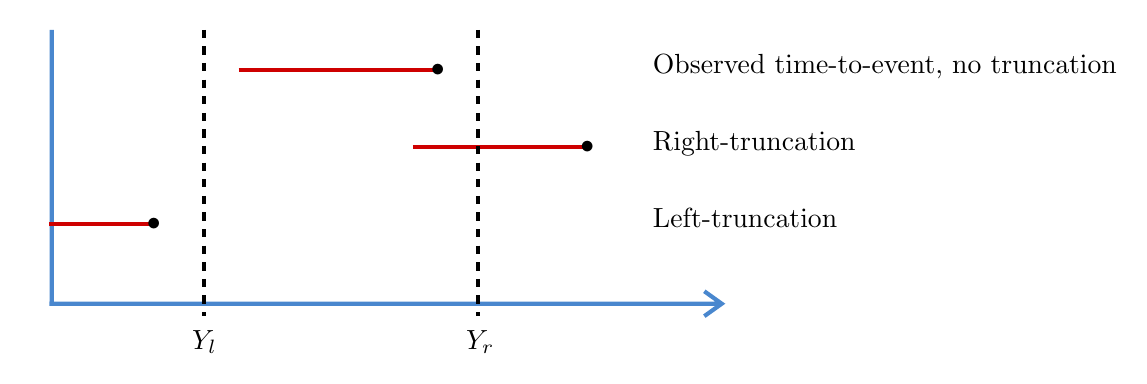
\begin{tikzpicture}[x=0.9pt,y=0.9pt,yscale=-1,xscale=1]
        \path (70,200); %set diagram left start at 0, and has height of 200

        %Shape: Axis 2D [id:dp048941842347560494] 
        \draw [color={rgb, 255:red, 73; green, 135; blue, 206 }, draw opacity=1 ][line width=1.5][-]
        % axes
        (78.67,180.33) -- (348.67,180.33)
        (79.67,70.33) -- (79.67,180.33)

        % arrow
        (341.67,175.33) -- (348.67,180.33) -- (341.67,185.33);

        \draw;

        \draw [color={rgb, 255:red, 206; green, 0; blue, 0 }, draw opacity=1][line width=1.5][-]

        (78.67,148.33) -- (120.67,148.33)
        (224.67,117.33) -- (294.67,117.33)
        (154.67,86.33) -- (234.67,86.33);

        \draw;

        \draw [color={rgb, 255:red, 0; green, 0; blue, 0 }, draw opacity=1][line width=1.5][-][dashed]
        % reporting date
        (250.67,70.33) -- (250.67,185.33)
        (140.67,70.33) -- (140.67,185.33);
        \draw;

        \draw [-] (135,190) node [anchor=north west][inner sep=0.75pt] [align=left] {$Y_l$};
        \draw [-] (245,190) node [anchor=north west][inner sep=0.75pt] [align=left] {$Y_r$};

        \draw [-] (320,79) node [anchor=north west][inner sep=0.75pt] [align=left] {Observed time-to-event, no truncation};
        \draw [-] (320,110) node [anchor=north west][inner sep=0.75pt] [align=left] {Right-truncation};
        \draw [-] (320,141) node [anchor=north west][inner sep=0.75pt] [align=left] {Left-truncation};

        % dots
        \foreach \Point in {
                (120.67,148.66),
                (294.67,117.66),
                (234.67,86.66)}{
                \node at \Point {$\bullet$};
            }

    \end{tikzpicture}
    \caption[Examples of left and right-truncation for patients in time-to-event data]{Examples of left and right-truncation for patients in time-to-event data, assuming only information within the truncation interval $(Y_l, Y_r)$ is observed. $Y_l$: left-truncation time, $Y_r$: right-truncation time, $\bullet$: outcome time.}\label{fig:truncation}
\end{figure}